% With the observation that ribosomes set an inherent upper limit on growth
% rate, through both rRNA synthesis and the additional dependence on ribosomal
% fraction, it is also plausible that ribosomes may play a more dominant role
% in setting growth rate across other growth conditions. With a rich proteomic
% data set across a wide array of conditions, and in light of a number of
% recent experimental observations, we find that cells also appear to tune
% their ribosomal abundance as a means to maximize growth even in poor nutrient
% conditions. This has important consequences on the relationship with cell
% size and maintenance of steady-state growth. In the coming section and the
% remainder of the text, we consider these further beginning with cell size.

\subsection{Relationship Between Cell Size and Growth Rate}
The relationship
between cell size and growth rate has long been of interest in the study of
bacterial physiology, particularly following the now six decade-old observation
that cell volume appears to increase exponentially with growth rate; known as
Schaechter's growth law  \citep{schaechter1958, taheriaraghi2015}. However, the
mechanism that governs this relationship, and even the question of whether the
change in average cell size is truly exponential has remained under debate
\citep{harris2018}. Given the importance of cell size in determining the total
protein mass that must be doubled and in setting other parameters like the
surface-area-to-volume ratio, we examine the proteomic data presented thus far
data to consider cell size and growth rate.

At moderate growth rates (above about 0.5 hr$^{-1}$), cells grow at a near-maximal rate near given their ribosomal
mass fraction $\Phi_R$ (\FIG{ribosome_limit}(B)). This means that in order to grow any faster, cells must
increase $\Phi_R$ further. A na\"ive strategy following the constraint of
\EQ{translation_limit_growth_rate} is simply that cells should make additional  ribosomes. In reality, however, large swaths of the proteome
increase in absolute protein abundance as cells grow faster (Supplemental Figure
X), and the ability to add additional ribosomes is likely constrained by other
factors including crowding due to their large size \citep{delarue2018,
solerbistue2020}. Instead, it is well-documented that \textit{E. coli} cells add
a constant volume per origin of replication,
which is robust to a remarkable array of cellular perturbations \citep{si2017}.
To consider this in the context of the proteomic data, we used the measurements from
\cite{si2017} for wild-type \textit{E. coli} cells grown in different nutrient conditions
(\FIG{translation_ecoli_partA}(A)) to estimate the average number of origins per cell $\langle$\# ori$\rangle$ across the data. Indeed, we find an approximately linear trend between protein
copy number and $\langle$\# ori$\rangle$, and in \FIG{translation_ecoli_partA}(B) plot
this for ribosomal copy numbers.

The average number of origins $\langle$\# ori$\rangle$ is set by how often
replication must be initiated per cell doubling under steady-state growth,
and can be quantified via
\begin{equation}
    \langle \text{\# ori} \rangle = 2^{\tau_{cyc} / \tau} = 2^{\tau_{cyc} \lambda / ln(2)},
    \label{eq:Nori}
\end{equation}
where $t_{cyc}$ is the cell cycle time (referring to the time from replication
initiation to cell division), and $\tau$ is the cell doubling time. For a
constant cell cycle time, observed at growth rates above about 0.5 hr$^{-1}$
\citep{helmstetter1968}, \EQ{Nori} says that $\langle \text{\# ori} \rangle$ will increase
exponentially with the growth rate.


% Wild-type
% \textit{E. coli} growing at relatively fast growth rates exhibit a remarkably
% constant cell cycle time $t_{cyc}$ (referring to the C and D periods of DNA
% replication and cell division, respectively), as shown in
% \FIG{translation_ecoli_partA}(A) for the data reproduced from \cite{si2017}.
% With a constant cell cycle time, the exponential scaling in size has most recently been
% considered a direct consequence of cells initiating replication at a constant
% volume per origin.
% However, the particular mechanism that governs this
% relationship, and even the question of whether the change in average cell size
% is truly exponential  have remained under debate \citep{si2017, harris2018}.

% Since protein accounts for more than half of cellular dry mass (BNID: 104954,
% \cite{milo2010, bremer2008, basan2015}, cell size will vary in proportion to how
% much protein is synthesized over the cell cycle.  Through our estimates in the
% sections on the central dogma, it is apparent that the processes of
% transcription (i.e. synthesis of mRNA) and translation are unlikely limiting
% steps in doubling the cell mass. In both cases, there is an overabundance of the
% requisite protein complexes (DNA and RNA polymerase, respectively) and there are
% mechanisms by which these synthesis processes can be parallelized. Therefore,
% the total protein mass is determined by $r_t \times R$ and the doubling time
% $\tau$. The relationship between cell size and growth rate, however, will depend
% only on how the cell scales its ribosomal fraction $\Phi_R$, as highlighted by
% \EQ{translation_limit_growth_rate}.


% \subsubsection{Exponential Scaling of Cell Size
% Follows from a need to Increase Absolute Ribosomal Abundance.}



%
% Wild-type \textit{E. coli} growing at relatively fast growth rates exhibit a
% remarkably constant cell cycle time $t_{cyc}$ (referring to the C and D periods
% of DNA replication and cell division, respectively), as shown in
% \FIG{translation_ecoli_partA}(A) for the data reproduced from \cite{si2017}.
% With a constant cell cycle time, the exponential scaling in size has most
% recently been considered a direct consequence of cells initiating replication at
% a constant volume per origin. This was found valid across a substantial number
% of  growth perturbations, highlighting that it is the relationship between cell
% size  and number of chromosomal origins of replication, $\langle\text{\#
% ori}\rangle$, that the cell maitains.



%  empirical evidence has
% revealed a linear scaling between cell size (volume) and the number of
% chromosomal origins of replication, $\langle\text{\# ori}\rangle$, which is
% robust to a remarkable array of perturbations \citep{si2017}.


% From \EQ{translation_limit_growth_rate}, we expect that both
% the number of
% ribosomes $R$ and $N_{aa}$ will vary in proportion to  $\langle$\# ori$\rangle$.
% It is only because $\Phi_R$ varies with $\langle$\# ori$\rangle$, that we observe
% an exponential
%
% growth rate that the increases to a greater extent than $N_{aa}$ with $\langle$\# ori$\rangle$
% that there will be anyHere we note that it  is only if the number of ribosomes
% per cell increases  to
%
% In order to relate changes in cell size with growth rate we need
% to consider how ribosomal content varies with $\langle$\# ori$\rangle$.
% [It is notable that in \textit{E. coli}, the
% majority of ribosomal proteins and rRNA operons are found closer to the origin
% of replication. Since multiple rounds of DNA initiation will effectively skew
% gene dosage in favor of genes near the origin \citep{scholz2019}, it suggests
% that an increase in  $\langle$\# ori$\rangle$ is a means to skew the ribosomal
% fraction of the proteome, $\Phi_R$.

Insight into why cells add a constant volume per $\langle$\# ori$\rangle$, and
how this relates to growth, however, requires us to consider the changes in the
proteome, and in particular ribosomal proteins across the different growth
conditions. In \FIG{translation_ecoli_partA}(D) we consider the
position-dependent protein expression across the chromosome for each of the
growth conditions from \cite{schmidt2016}. Here we calculated a running
Gaussian average of protein copy number (20 kbp st. dev. averaging window) based on each gene's transcriptional start site, which were then
median-subtracted to account for the differences in total protein abundance with each
growth condition. Importantly, we find that the major deviations in protein copy
number are largely restricted to regions of ribosomal protein genes, with
substantially higher deviations observed for cells with high $\langle$\#
ori$\rangle$ (teal), as compared to those with low $\langle$\# ori$\rangle$
(purple). This is particularly apparent for genes closer to the origin, where
the majority of ribosomal proteins are found. This suggests that in addition
to the linear scaling between protein abundance and $\langle$\# ori$\rangle$,
cells are also varying their relative ribosomal abundance in proportion to
$\langle$\# ori$\rangle$. Since growth rate depends specifically on the
ribosomal fraction $\Phi_R$, this result suggests that cells are changing their
size as a way to tune $\Phi_R$ to match the available nutrient conditions.


% It is this relationship in particular that leads to an
% exponential relationship between cell size and growth rate under
% nutrient-limited growth. Said differently, if cells added a constant volume per
% $\langle$\# ori$\rangle$  but maintained a constant $\Phi_R$,  no
% longer exhibit a change in this exponential relationship between cell size and
% growth rate.



\begin{figure*}
    \begin{fullwidth}
    \centering{
        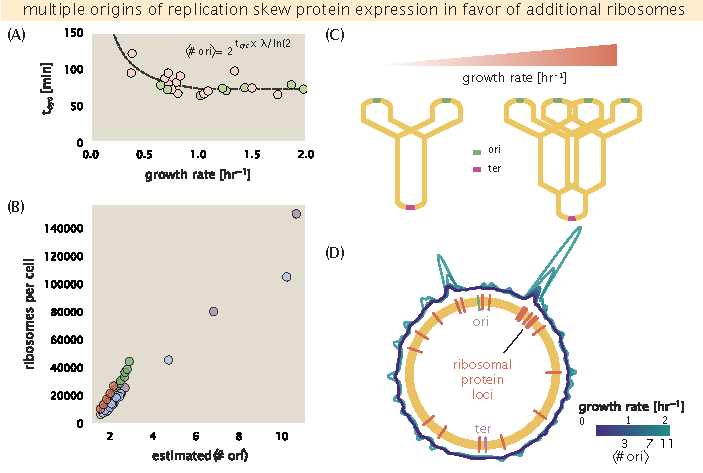
\includegraphics{main_figs/fig8_ribosome_growth_limit_ecoli_a_polar_coord.pdf}
        \caption{\textbf{Multiple replication initiations bias protein synthesis
        in favor of more ribosome.} (A) Experimental data from Si \textit{et al.}
        (2017). Dashed line shows fit to the data, which were used to estimate
        $\langle$\# ori$\rangle$. $t_{cyc}$ was assumed to vary in proportion to
        $\tau$ for doubling times great than 40 minutes, and then reach a
        minimum value of [fill in] minutes below this (see Supplemental Appendix
        X for additional details). Red data points correspond to measurements in
        strain MG1655, while light green points are for strain NCM3722. (B) Plot
        of the ribosome copy number estimated from the proteomic data against
        the estimated $\langle$\# ori$\rangle$. (C) Schematic shows the expected increase in replication
        forks (or number of ori regions) as \textit{E. coli} cells grow faster.
        (D) A running Gaussian average (20 kbp st. dev.) of protein copy number is calculated for
        each growth condition considered by \citep{schmidt2016}. Since total
        protein abundance increases with growth rate, protein copy
        numbers are median-subtracted to allow comparison between growth conditions.
        $\langle$\# ori$\rangle$ are estimated using the data in (A) and Equation \ref{eq:Nori}.
        [still looking into how best to use this type of analysis] } \label{fig:translation_ecoli_partA}
    }
    \end{fullwidth}
\end{figure*}



% genes closer to the origin that allows change the proteomic composition and allows an
% increase in the ribosomal fraction $\Phi_R$ at fast growth. For \textit{E.
% coli}, we can then view the increase in ribosomal fraction $\Phi_R$ (and
% therefore, $\lambda$) as requiring a geometric increase in total protein
% abundance that is proportional to $\langle$\# ori$\rangle$. This leads to an
% exponential increase in total protein mass (and cell size) as long as all
% ribosomes $R$ are actively translating protein during cell doubling.

While this dependence between cell size and ribosomal abundance is apparent across
moderate to fast growth rates, it is worth noting that this scaling
is likely to change at slow growth rates (below $\lambda \approx
0.5\,\text{hr}^{-1}$). Here, the number of ribosomes $R$ no longer reflects the
cell's protein synthesis capacity \citep{dai2016}, so far taken to be $r_t
\times R$, and instead, cells have an excess number of ribosomes. Additional regulatory
control through the small-molecule alarmones such as guanosine pentaphosphate
[(p)ppGpp] reduce the fraction of actively translating ribosomes
at these slower growth rates. This overabundance of ribosomes
provides different challenges on the ability of the cell to maintain steady-state
growth under limiting nutrient conditions, and in Supplemental
Section XX we consider this slow growth regime further.
% This is why \cite{si2017} found that it was the change in active
% ribosomal fraction, and not ribosomal fraction alone, that was most consistent
% with an exponential change in cell size.


As a final comment, it has recently been shown that growth in a (p)ppGpp null
strain also lacked both the condition-dependent changes in $\langle$\#
ori$\rangle$ as well as changes in cell size across different growth condition.
Instead, cells always exhibited a high ratio of $\langle$\# ori$\rangle$ to
$\langle$\# ter$\rangle$, irrespective of growth rate, and a cell size that was
more consistent with a fast growth state where (p)ppGpp levels are normally low
\citep{fernandezcoll2020} and ribosomal fraction is high \citep{zhu2019}. There
is also evidence that this may be achived through inhibition of DNA replication
initiation \citep{kraemer2019}. These observations raise the possibility that
(p)ppGpp may be playing a causal role in tuning $\langle$\# ori$\rangle$ and
cell size, which ultimately allows the cell to vary its ribosomal content
according to nutrient availability.

[This last paragraph may be better placed in the discussion]

% The specific relationship between cell size and growth rate
% however becomes harder to define because cells no longer need multiple rounds of
% DNA replication to make enough rRNA, and no longer need to increase their total
% protein mass in order to tune protein synthesis. Our collated proteomic data,
% however, contain several assumptions that relate total protein abundance to
% growth rates and this prevents us from making precise predictions about how cell
% size and absolute protein abundance vary at slow growth (Supplemental X).
% Nevertheless, we find no evidence that cells decrease their size to the minimal
% value expected from on an exponential function with a constant exponent fit to
% cell sizes with moderate to fast growth rates \citep{basan2015, radzikowski2016,
% si2019}, suggesting at least a modified scaling between size and growth rate in
% these poorer nutrient conditions.
%
% \subsection{Growth in Poor Nutrient Conditions Requires Inhibition of Ribosomes.}
%
% In \FIG{}(B), we see that in the poorest nutrient conditions
% [NB: start by highlighting the dilemma when cells have excess ribosomes].
%
% How do cells regulate protein synthesis when amino acids become limiting,
% meaning that consumption exceeds the rate of synthesis? In the slowest  growth
% conditions, we find a minimum ribosomal mass fraction of $\Phi_R \approx 0.06$
% and  of order 10$^4$ ribosomes per cell.  Without the additional regulatory
% control noted above, there would be a point where  this imbalance would occur if
% all ribosomes were actively translating  (\FIG{translation_ecoli_partB}). Such a
% scenario would prevent continuous growth, and indeed for (p)ppGpp null strains,
% cells only grow in minimal media if additional amino acid supplements are
% present. In contrast, wild-type \textit{E. coli} maintain a relatively high
% elongation rate even in stationary phase ($\approx$ 8 AA/s, \citep{dai2016,
% dai2018}).
%
% To better understand how regulation of ribosomes influence growth rate at
% slow growth, we consider a coarse-grained model that relates elongation
% rate to a limiting supply of amino acids, which for simplicity we treat as a
% single, effective rate-limiting species $[AA]_{eff}$. Under such a scenario, the elongation
% rate $r_t$ can be described as depending on the maximum elongation rate ($r_t^{max}
% \approx$ 17.1 AA/s, \citep{dai2016, dai2018}), an effective binding constant
% $K_D$ between the pool of amino acids and their amino-acyl tRNAs, and the limiting
% amino acid concentration $[AA]_{eff}$,
%
% \begin{equation}
% r_t = r_t^{max} \cdot \frac{1}{1 + K_D / [AA]_{eff}}.
% \label{eq:rate_Kd}
% \end{equation}
% For cells growing in minimal medium supplemented with glucose, the amino acid
% concentration is of order 100 mM (BNID: 110093, \citep{milo2010, bennett2009}).
% To estimate  $K_D$, we note that for a growth rate of about 0.6 hr$^{-1}$
% \cite{dai2016} measured an elongation rate of about 12.5 AA$\cdot$s$^{-1}$,
% yielding $K_D \approx 40$ mM. The maintenance of this amino acid pool
% $[AA]_{eff}$ will depend on the difference between the synthesis/supply rate of
% amino acids $r_{AA}$ and consumption by ribosomes $r_t \times R \times f_a$,
% where we use $f_a$ to account for the possible reduction of actively translating
% ribosomes (see Supplemental Appendix XX for further details on this model).
%
% In \FIG{translation_ecoli_partB}(B), we show the relationship between the growth
% rate and elongation rate as a function of the number of actively translating
% ribosomes. Here, growth rate is now determined by the active ribosomal fraction via
% \begin{equation}
% \lambda_\text{translation-limited} \approx \frac{r_t}{L_R}  \Phi_R f_a.
% \label{eq:translation_limit_growth_rate_2}
% \end{equation}
% If we consider constant values of amino acid synthesis rate $r_{AA}$ (dashed
% lines) to reflect the available parameter space for a specific growth condition,
% the fastest growth rates result from  maximization of the fraction of actively translating
% ribosomes. When we consider the experimental measurements from \cite{dai2018}
% (yellow circles), reflecting growth in different nutrient conditions, we see
% that although $R \times f_a$ is reduced in poorer nutrient conditions, it is
% reduced in a manner such that $[AA]_{eff}$ is relatively constant. Given our estimate
% $K_D \approx$ 40 mM,  we would only expect a decrease from 100 mM to about 35 mM
% in the slowest growth conditions. While experimental data is scarce, data from
% \cite{bennett2009} show that amino acid
% concentrations only decrease to about 60 mM for cells grown in minimal media
% supplemented with acetate ($\lambda \approx$  0.3 hr$^{-1}$ in our proteomic data)
% \citep{bennett2009}, qualitatively consistent with our expectations. One
% explanation for the experimental data is that the active fraction of the
% ribosome pool is regulated in order to maintain a sufficient supply of amino acids for
% growth. Any further increase in $R \times f_a$ at constant $r_{AA}$ would
% otherwise be associated with an additional drop in cellular amino acid
% concentration.
%
% \begin{figure*}
%     \begin{fullwidth}
%     \centering{
%         \includegraphics{main_figs/fig8_ribosome_growth_limit_ecoli_b.pdf}
%         \caption{\textbf{\textit{E. coli} must regulate ribosomal activity in
%         limiting nutrient conditions. }
%         (A) Schematic showing translation-specific requirements for maintenance
%         of steady-state growth. In a nutrient rich environment, amino acid
%         supply $r_{aa}$ is sufficiently in excess of the demand by ribosomes
%         translating at their maximal rate. In poorer nutrient conditions,
%         reduced amino acid supply $r_{aa}$ will decrease the rate of elongation.
%         In a regime where $r_{aa}$ is less than $r_tR$, the number of
%         actively translating ribosomes will need to be reduced in order to
%         maintain steady-state growth. (B) Translation elongation rate is plotted
%         as a function of the number of actively translating ribosomes $R
%         f_a$. Dashed lines correspond to a range of amino acid synthesis rates
%         $r_{aa}$, from 10$^3$ to 10$^6$. Growth rates are calculated according
%         to Equation 1, assuming a constant ribosomal fraction of 8 percent. See
%         appendix XX for additional details. (C) Experimental data from \citep{dai2016}
%         are used to estimate the fraction of actively translating ribosomes. The solid line represents the translation-limited
%         growth rate for ribosomes elongating at 17.1 AA/s.}
%         \label{fig:translation_ecoli_partB}
%     }
%     \end{fullwidth}
% \end{figure*}
%
%
% \subsection{\textit{E. coli} Maintains Steady-State Growth
% Rate by Tuning both Ribosomal Content and Translation Activity.}
% Using the active fraction $f_a$ measurements across a broad range of
% nutrient-limited growth conditions from the work of \cite{dai2016}, we
% furthermore estimated the active fraction of ribosomal protein across the
% collated proteomic datasets (\FIG{translation_ecoli_partB}(C)). Importantly, we
% note that across all growth conditions considered, cells appear to maintain a
% growth rate consistent with \EQ{translation_limit_growth_rate} with an
% elongation rate of $r_t \approx$  17.1 AA/s. While somewhat counter intuitive,
% given that ribosomes translate at almost half this rate in the poorest of growth
% conditions, steady-state growth rates can be achieved over such a broad range of
% conditions because cells have evolved a means to tune  $r_t \times R \times
% f_a$.
%
% It has recently been shown that growth in a (p)ppGpp null strain abolishes both
% the the growth-dependent changes in gene dosage and  scaling in cell size.
% Instead, cells always exhibited a higher gene dosage near  near the origin of
% replication, irrespective of growth rate, and a cell size more consistent with a
% fast growth state where (p)ppGpp levels are low \citep{fernandezcoll2020} and
% ribosomal fraction is high \citep{zhu2019}. This raises the possibility that the
% action of (p)ppGpp is also mediating growth control and size scaling over the
% entire range of growth conditions. Specifically, as nutrient conditions worsen,
% (p)ppGpp acts to also inhibit DNA replication initiation \citep{kraemer2019}
% helps decrease multiple rounds of DNA replication per cell doubling which
% effectively decreases both $R$ and the total cell size \textit{and} in
% sufficiently poor growth conditions mitigates translation activity according to
% nutrient availability.
